\documentclass[]{elsarticle} %review=doublespace preprint=single 5p=2 column
%%% Begin My package additions %%%%%%%%%%%%%%%%%%%

\usepackage[hyphens]{url}

  \journal{Data Mining} % Sets Journal name

\usepackage{lineno} % add

\usepackage{graphicx}
%%%%%%%%%%%%%%%% end my additions to header

\usepackage[T1]{fontenc}
\usepackage{lmodern}
\usepackage{amssymb,amsmath}
\usepackage{ifxetex,ifluatex}
\usepackage{fixltx2e} % provides \textsubscript
% use upquote if available, for straight quotes in verbatim environments
\IfFileExists{upquote.sty}{\usepackage{upquote}}{}
\ifnum 0\ifxetex 1\fi\ifluatex 1\fi=0 % if pdftex
  \usepackage[utf8]{inputenc}
\else % if luatex or xelatex
  \usepackage{fontspec}
  \ifxetex
    \usepackage{xltxtra,xunicode}
  \fi
  \defaultfontfeatures{Mapping=tex-text,Scale=MatchLowercase}
  \newcommand{\euro}{€}
\fi
% use microtype if available
\IfFileExists{microtype.sty}{\usepackage{microtype}}{}
\usepackage[]{natbib}
\bibliographystyle{plainnat}

\usepackage{graphicx}
\ifxetex
  \usepackage[setpagesize=false, % page size defined by xetex
              unicode=false, % unicode breaks when used with xetex
              xetex]{hyperref}
\else
  \usepackage[unicode=true]{hyperref}
\fi
\hypersetup{breaklinks=true,
            bookmarks=true,
            pdfauthor={},
            pdftitle={ Actividad Evaluativa \#1 Grupo 5 Universidad Andrés Bello Facultad de Ingeniería Ingeniería Civil Informática Ingeniería Civil Industrial},
            colorlinks=false,
            urlcolor=blue,
            linkcolor=magenta,
            pdfborder={0 0 0}}

\setcounter{secnumdepth}{0}
% Pandoc toggle for numbering sections (defaults to be off)
\setcounter{secnumdepth}{0}


% tightlist command for lists without linebreak
\providecommand{\tightlist}{%
  \setlength{\itemsep}{0pt}\setlength{\parskip}{0pt}}



\usepackage{float}
\usepackage{booktabs}
\usepackage{longtable}
\usepackage{array}
\usepackage{multirow}
\usepackage{wrapfig}
\usepackage{float}
\usepackage{colortbl}
\usepackage{pdflscape}
\usepackage{tabu}
\usepackage{threeparttable}
\usepackage{threeparttablex}
\usepackage[normalem]{ulem}
\usepackage{makecell}
\usepackage{xcolor}



\begin{document}


\begin{frontmatter}

  \title{
\includegraphics[width=1.5625in,height=1.5625in]{logo_UNAB.png}\\
Actividad Evaluativa \#1\\
Grupo 5\\
Universidad Andrés Bello\\
Facultad de Ingeniería\\
Ingeniería Civil Informática\\
Ingeniería Civil Industrial}
    \author[]{Martín Fernández 1%
  %
  \fnref{1}}
   \ead{nombre@uandresbello.edu} 
    \author[]{Tomás Moya 2}
   \ead{nombre@uandresbello.edu} 
    \author[]{Wesly Ocampo 3%
  %
  \fnref{2}}
   \ead{nombre@uandresbello.edu} 
    \author[]{Alan Tovar 4%
  %
  \fnref{3}}
   \ead{nombre@uandresbello.edu} 
      \cortext[cor1]{Corresponding author}
  
  \begin{abstract}
  Describir brevemente en qué consiste este primer análisis de los
  datos, e incluir el objetivo del estudio. (máximo 150 palabras)
  \end{abstract}
  
 \end{frontmatter}

\newpage

\section{Introducción}

El preprocesamiento de datos y la administración de los mismos nos
permiten la recolección de datos de distintas fuentes, el tratamiento de
filas y cabeceras (headers o columnas). Con esto podemos hacer una
limpieza adecuada, eliminar errores, corregir inconsistencias y aumentar
la calidad de la minería de datos, una correcta gestión de datos también
nos sirve para acceder a diferentes datos de una forma más fácil, así
obtenemos información estadística y comparativa que permite una correcta
toma de decisiones y abarcar de mejor manera los distintos problemas
empresariales.

En este caso nuestra base de datos es de una renta de bicicletas que
cuenta con 5856 observaciones clasificadas en las siguientes 14
variables con su tipo de variable correspondiente:

\begin{enumerate}
\def\labelenumi{\arabic{enumi}.}
\tightlist
\item
  Fecha (Categórica)
\item
  Recuento de bicicletas alquiladas (Numérica)
\item
  Hora (Numérica)
\item
  Temperatura (Numérica)
\item
  Humedad (Numérica)
\item
  Velocidad del viento (Numérica)
\item
  Visibilidad (Numérica)
\item
  Temperatura de punto de rocío (Numérica)
\item
  Radiación solar (Numérica)
\item
  Lluvia (Numérica)
\item
  Nevada (Numérica)
\item
  Estaciones (Categórica)
\item
  Vacaciones (Categórica)
\item
  Día de funcionamiento (Categórica)
\end{enumerate}

Nuestro objetivo es analizar esta base de datos, variables categóricas y
numéricas para ver su distribución, determinar si hay datos atípicos,
datos faltantes y ver como se relacionan las distintas variables entre
sí.

\newpage
\section{Desarrollo}

\subsection{Resumen de medidas estadísticas}

\ref{tab:tab1} \newpage

\begin{table}

\caption{\label{tab:tab1}\label{tab:tab1}Resumen de medidas estadísticas.}
\centering
\begin{tabular}[t]{l|r|r|r|r|r|r|r|r|r}
\hline
variables & min & Q1 & mean & median & Q3 & max & zero & minus & outlier\\
\hline
Rented\_Bike\_Count & 0 & 327.75 & 905.83 & 813.00 & 1298.50 & 3556.00 & 295 & 0 & 55\\
\hline
Hour & 0 & 5.75 & 11.50 & 11.50 & 17.25 & 23.00 & 244 & 0 & 0\\
\hline
Temperature & -3 & 12.90 & 19.19 & 19.90 & 25.20 & 39.40 & 1 & 21 & 0\\
\hline
Humidity & 0 & 46.00 & 61.22 & 61.00 & 77.00 & 98.00 & 17 & 0 & 0\\
\hline
Windspeed & 0 & 0.90 & 1.63 & 1.50 & 2.20 & 7.40 & 48 & 0 & 100\\
\hline
Visibility & 27 & 1003.00 & 1470.78 & 1731.00 & 2000.00 & 2000.00 & 0 & 0 & 0\\
\hline
Dew\_point\_temperature & -19 & 4.10 & 10.71 & 11.40 & 18.70 & 27.20 & 43 & 726 & 3\\
\hline
Solar\_Radiation & 0 & 0.00 & 0.67 & 0.05 & 1.17 & 3.52 & 2664 & 0 & 196\\
\hline
Rainfall & 0 & 0.00 & 0.20 & 0.00 & 0.00 & 35.00 & 5392 & 0 & 464\\
\hline
Snowfall & 0 & 0.00 & 0.02 & 0.00 & 0.00 & 8.80 & 5805 & 0 & 51\\
\hline
\end{tabular}
\end{table}

\subsection{Análisis de la variable Seasons}

En la figura \ref{fig:fig1} solo tiene 3 estaciones, podemos asumir que
no existe recolección de datos durante el invierno debido a las
características climáticas, presentando un clima demasiado frió y con
posible nieve que son razones por las cuales los clientes no quieran
rentan bicicletas y que la empresa no opere durante ese tiempo por las
nulas ganancias.

\begin{figure}[H]

{\centering 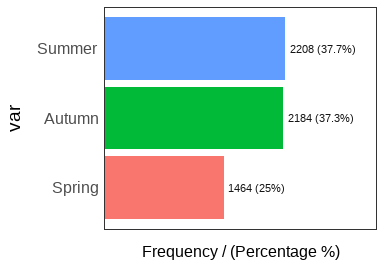
\includegraphics[width=1\linewidth]{barplot_seasons} 

}

\caption{\label{fig:fig1}Histograma de Seasons.}\label{fig:fig1}
\end{figure}

\subsection{Análisis de la variable Bicicletas Rentadas Rented Bike Count}

\newpage
\begin{table}

\caption{\label{tab:tab2}\label{tab:tab2}Tabla de frecuencias de Bicicletas Rentadas Rented Bike Count.}
\centering
\begin{tabular}[t]{l|l|r|r|r|r}
\hline
variables & levels & N & freq & ratio & rank\\
\hline
Rented\_Bike\_Count & (140,160] & 641 & 91 & 14.20 & 1\\
\hline
Rented\_Bike\_Count & (20,40] & 641 & 87 & 13.57 & 2\\
\hline
Rented\_Bike\_Count & (160,180] & 641 & 82 & 12.79 & 3\\
\hline
Rented\_Bike\_Count & (0,20] & 641 & 80 & 12.48 & 4\\
\hline
Rented\_Bike\_Count & (120,140] & 641 & 75 & 11.70 & 5\\
\hline
Rented\_Bike\_Count & (40,60] & 641 & 72 & 11.23 & 6\\
\hline
Rented\_Bike\_Count & (60,80] & 641 & 56 & 8.74 & 7\\
\hline
Rented\_Bike\_Count & (100,120] & 641 & 54 & 8.42 & 8\\
\hline
Rented\_Bike\_Count & (80,100] & 641 & 44 & 6.86 & 9\\
\hline
\end{tabular}
\end{table}

El gráfico del histograma con curva de densidad correspondiente a la
figura \ref{fig:fig3} podemos analizar que la mayoría de las frecuencias
está concentrada en los primeros intervalos, es decir la variable
presenta una asimetría positiva y una variación heterogénea, presentando
una tendencia a una mayor densidad mientras se esté más cerca del cero
mientras menos bicicletas hayan sido alquiladas

\begin{figure}[H]

{\centering 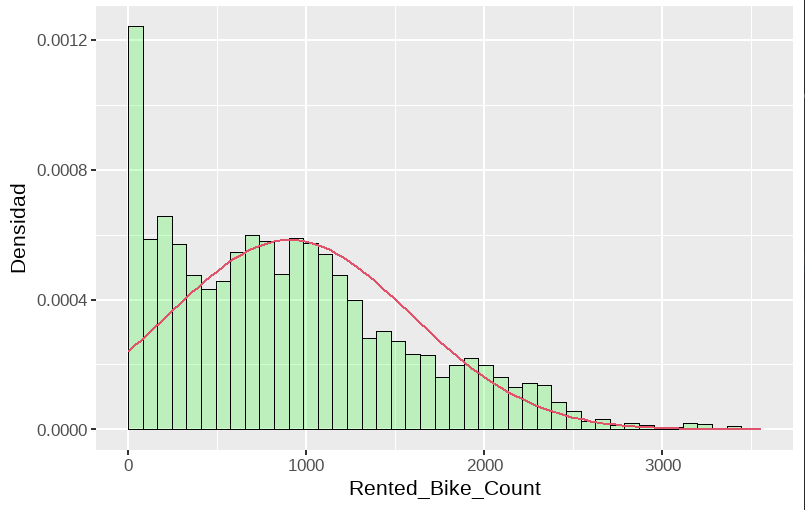
\includegraphics[width=1\linewidth]{frec_density} 

}

\caption{\label{fig:fig3}Histograma con curva de densidad de Bicicletas Rentadas Rented Bike Count.}\label{fig:fig3}
\end{figure}
\newpage

Según el gráfico Q-Q obtenido correspondiente a la figura \ref{fig:fig4}
se puede concluir que los datos en su mayoría mantienen una distribución
asimétrica positiva.

\begin{figure}[H]

{\centering 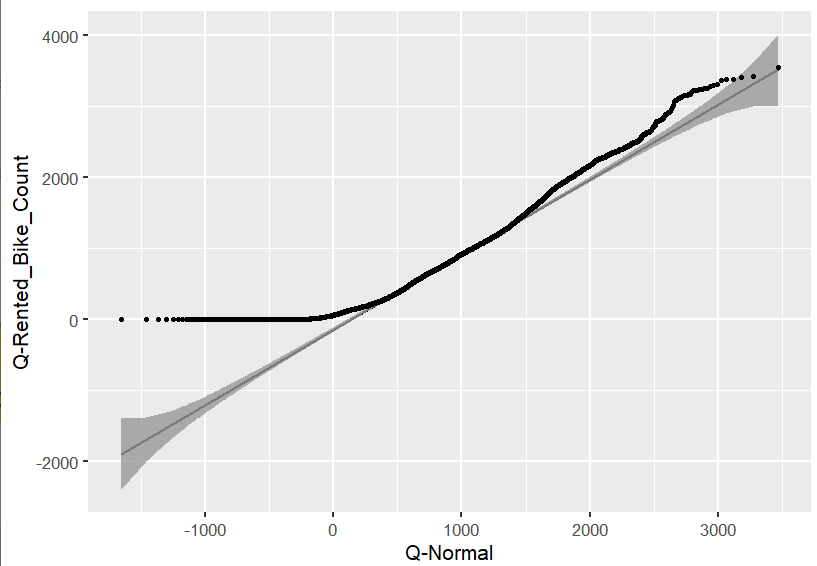
\includegraphics[width=1\linewidth]{qq} 

}

\caption{\label{fig:fig4}Q-Q plot de Bicicletas Rentadas Rented Bike Count.}\label{fig:fig4}
\end{figure}

Segun el test de kolmogorov-smirnov de la variable bicicletas rentadas
el valor de probabilidad es menor a 2.2e-16. Por ende rechazamos la
hipótesis nula al ser nuestro valor no mayor a 0.05, es decir la
distribución no es normal.

\begin{verbatim}
## 
##  Asymptotic one-sample Kolmogorov-Smirnov test
## 
## data:  datos$Rented_Bike_Count
## D = 0.092264, p-value < 2.2e-16
## alternative hypothesis: two-sided
\end{verbatim}

\newpage
\subsection{Valores Atípicos}

En este gráfico de boxplot correspondiente a la figura \ref{fig:fig5}
observamos los datos atípicos, en esta variable previamente vimos que
teníamos 55 datos atípicos, todos son superiores, no tenemos datos
atípicos inferiores y se encuentran en un rango entre 2500 y 4000
aproximadamente.

\begin{figure}[H]

{\centering 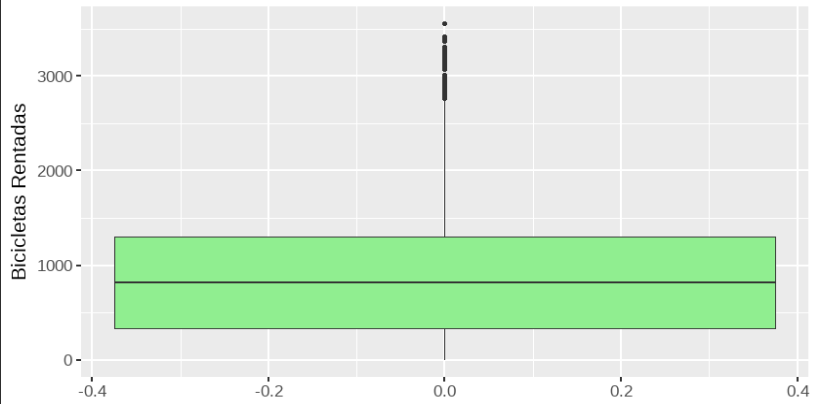
\includegraphics[width=1\linewidth]{datos_atypical} 

}

\caption{\label{fig:fig5}Datos Atípicos de Bicicletas Rentadas Rented Bike Count. }\label{fig:fig5}
\end{figure}
\newpage

En este caso el boxplot de la figura \ref{fig:fig6} relacionamos las
variables categórica y numérica estudiadas anteriormente, aquí podemos
observar las bicicletas rentadas según la estación Podemos concluir que
todas las estaciones tienen valores atípicos y si vemos las medianas
sabremos que en verano se rentan más bicicletas.

\begin{figure}[H]

{\centering 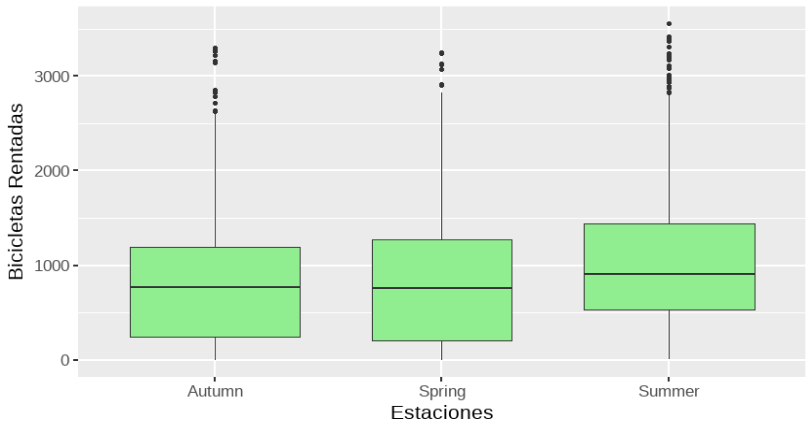
\includegraphics[width=1\linewidth]{boxplot_seasons} 

}

\caption{\label{fig:fig6}Boxplot de la variable Seasons. }\label{fig:fig6}
\end{figure}
\newpage
\subsection{Datos Faltantes}

Determinar proporción de datos faltantes

En este gráfico de proporcion de datos faltantes, figura
\ref{fig:fig7}podemos observar que ninguna variable de nuestra base de
datos tiene datos perdidos. Por ende no es necesario realizar ninguna
imputación

\begin{figure}[H]

{\centering 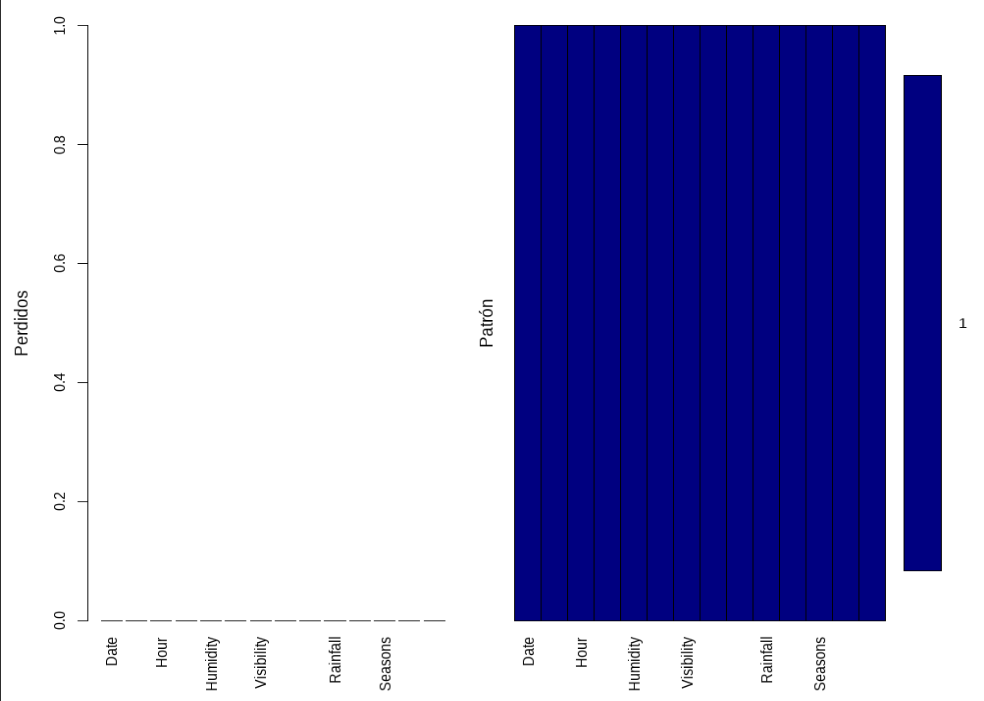
\includegraphics[width=1\linewidth]{missing_data} 

}

\caption{\label{fig:fig7}Gráfico de Datos faltantes.}\label{fig:fig7}
\end{figure}
\newpage
\subsection{Análisis de Correlación}

En este grafico correspondiente a la figura \ref{fig:fig8} podemos
observar cómo se relacionan entre si las variables de nuestra base de
datos, es decir, que tanto afecta una a la otra. En el caso de nuestra
base de datos podemos observar Correlación nula o despreciable entre
Temperatura de rocío y bicicletas alquiladas, hora, velocidad del
viento, radiación solar, también entre Lluvia y hora, temperatura,
velocidad del viento y entre Radiación solar y visibilidad Por otro
lado, con Correlación fuerte positiva tenemos a Temperatura de rocío y
temperatura, humedad o a Bicicletas alquiladas y hora Por último,
tenemos Correlación fuerte negativa entre Humedad y radiación solar,
visibilidad, bicicletas rentadas.

\begin{figure}[H]

{\centering 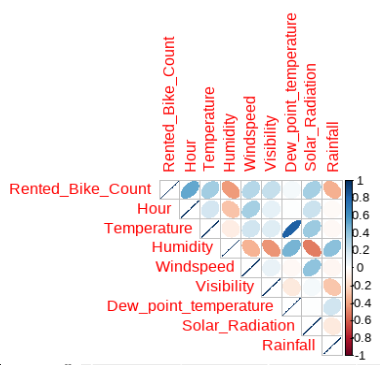
\includegraphics[width=1\linewidth]{corr} 

}

\caption{\label{fig:fig8}Matriz de Correlación.}\label{fig:fig8}
\end{figure}
\newpage
\section{Conclusiones}

Resuma las principales conclusiones de cada análisis realizado como
parte del desarrollo.

Luego de este análisis podemos concluir que el análisis exploratorio de
datos es indispensable para organizar los datos, entender su contenido,
visualizar y extraer información relevante del set de datos para poder
decidir cuál será la técnica más adecuada para procesarlos
posteriormente. En el caso de nuestra base de datos definimos sus
variables, sus tipos, luego del análisis de la variable bicicletas
rentadas concluimos que su distribución es asimétrica positiva, como se
relacionaban las variables entre sí, no teníamos datos faltantes,
contábamos con datos atípicos en algunas variables, no contábamos con
datos en invierno por lo que creemos que la empresa no trabajaba en esta
estación ya que es muy difícil transportarse en bicicleta en climas
extremadamente bajos y también pudimos ver que en el verano se rentaba
una mayor cantidad de bicicletas.


\end{document}
